% created on 2019-12-13
% @author : bmazoyer

%% Lines to compile only this capter
\documentclass[11pt, twoside, a4paper, openright]{report}
\usepackage[utf8]{inputenc}
% \DeclareUnicodeCharacter{223C}{~}

%Bibliography style
% \usepackage[square, numbers]{natbib}
% \usepackage[round]{natbib}
% \usepackage{biblatex}
% \bibliographystyle{unsrtnat}
% \bibliographystyle{unsrt}
% \bibliographystyle{plain}
% \bibliographystyle{aa}
% \usepackage[backend=bibtex,style=authoryear,natbib=true]{biblatex} 
\usepackage[
backend=biber,
style=authoryear,
citestyle=authoryear,
url=false
]{biblatex}
\addbibresource{../source/library.bib}

\usepackage[T1]{fontenc}
\usepackage[french]{babel}
\usepackage{csquotes}  % used for citations (recommended when using biblatex)
%\usepackage{helvet}
%\renewcommand{\familydefault}{\sfdefault}
\usepackage{mathptmx}
\usepackage{amssymb}
\usepackage{geometry} 
\usepackage{xcolor}
\usepackage[absolute,overlay]{textpos}
\usepackage{graphicx}
\usepackage{lipsum}
\usepackage[explicit]{titlesec}
\usepackage{lmodern}
\usepackage{color}
\usepackage{array}
\usepackage{mathtools}
\usepackage{caption}
\usepackage{multicol}
\usepackage{booktabs}
\usepackage{enumitem}
\usepackage{hyperref}
\usepackage{afterpage}
\usepackage{emptypage}
\usepackage{setspace}
\usepackage{pgffor}
    \setlength{\columnseprule}{0pt}
    \setlength\columnsep{10pt}
\usepackage[francais,nohints]{minitoc}
    \setcounter{minitocdepth}{3}
 
 %https://la-bibliotex.fr/2019/02/03/ecrire-les-nombres-et-les-unites-avec-latex/   
\usepackage{siunitx}
% \sisetup{
%     detect-all,
%      output-decimal-marker={,},
%      group-minimum-digits = 3,
%      group-separator={~},
%      number-unit-separator={~},
%      inter-unit-product={~},
%      list-separator = {, },
%      list-final-separator = { et },
%      range-phrase = --,
%      separate-uncertainty = true,
%      multi-part-units = single,
%      list-units = single,
%      range-units = single
%     }
\usepackage{physics}
\usepackage{isotope}

\usepackage[perpage]{footmisc} % to reset the counter of footnote each page

    
\usepackage{fancyhdr}			% Entête et pieds de page. Doit être placé APRES geometry
\pagestyle{fancy}		% Indique que le style de la page sera justement fancy
%\lfoot[\thepage]{} 		% gauche du pied de page
%\cfoot{} 			% milieu du pied de page
%\rfoot[]{\thepage} 
\fancyfoot{} % vide le pied~de~page
\fancyfoot[LE,RO]{\thepage}
\fancyfoot[LO,CE]{}% droite du pied de page
\fancyhead{}	
\fancyhead[LE]{\leftmark}	
\fancyhead[RO]{\rightmark}

\fancypagestyle{plain}{%
\fancyhf{} % vide l’en-tête et le pied~de~page.
\fancyfoot[LE,RO]{\thepage} % numéro de la page en cours en gras% et centré en pied~de~page.
\renewcommand{\headrulewidth}{0pt}
\renewcommand{\footrulewidth}{0pt}}



% Premiere page des chapitres
\newlength\chapnumb
\setlength\chapnumb{3cm}
 
\titleformat{\chapter}[block] {
  \normalfont}{}{0pt} { %police
    \parbox[b]{\chapnumb}{
      \fontsize{120}{110}\selectfont\thechapter} %taille du chiffre
      \parbox[b]{\dimexpr\textwidth-\chapnumb\relax}{
        \raggedleft 
        \hfill{\bfseries\Huge#1}\\ %taille du titre
        \rule{\dimexpr\textwidth-\chapnumb\relax}{0.4pt} %ligne de separation
  }
}
 
 %premiere page chapitre non numerote (remerciement, table des matieres ...)
 
\titleformat{name=\chapter,numberless}[block]
{\normalfont}{}{0pt}
{   
    \parbox[b]{\dimexpr\textwidth}{%   
    \hfill{\bfseries\Huge#1}\\
  \rule{\dimexpr\textwidth}{0.4pt}}}
    
 %   \titleformat{name=\chapter,numberless}[block]
%{\normalfont}{}{0pt}
%{\parbox[b]{\chapnumb}{%
%   \mbox{}}%
%  \parbox[b]{\dimexpr\textwidth-\chapnumb\relax}{%
%    \raggedleft%
%    \hfill{\bfseries\Huge#1}\\
%    \rule{\dimexpr\textwidth-\chapnumb\relax}{0.4pt}}}


%%%    SIunitx
\sisetup{locale = FR,
  % inter-unit-product=\ensuremath{\cdot},
  inter-unit-product=\ensuremath{\,},
  per-mode=reciprocal,
  separate-uncertainty = true,
  detect-all
}
\DeclareSIUnit{\Mpc}{Mpc}
\DeclareSIUnit{\kpc}{kpc}
\DeclareSIUnit{\Gpc}{Gpc}
\DeclareSIUnit{\h}{\textit{h}~}
\DeclareSIUnit{\perh}{\textit{h}^{-1}\,}

%%% Geometry
\geometry{
left=20mm,
top=30mm,
right=20mm,
bottom=30mm
}

%%% Color
\definecolor{bordeau}{rgb}{0.3515625,0,0.234375}

%%% Commands
\newcommand{\Nmocks}{\num{30}}
\newcommand{\hMpc}{h^{-1}\,\mathrm{Mpc}}
\newcommand{\hGpc}{h^{-1}\,\mathrm{Gpc}}
\newcommand{\kms}{\mathrm{km\,s^{-1}}}

\newcommand{\lya}{Ly$\alpha$}
\newcommand{\lyb}{Ly$\beta$}
\newcommand{\lyalya}{Ly$\alpha$(Ly$\alpha$)}
\newcommand{\lyalyb}{Ly$\alpha$(Ly$\beta$)}

\newcommand{\lrf}{\lambda_{\rm RF}}
\newcommand{\kpar}{k_{\parallel}}
\newcommand{\apar}{\alpha_{\parallel}}
\newcommand{\rpar}{r_{\parallel}}
\newcommand{\aperp}{\alpha_{\perp}}
\newcommand{\rperp}{r_{\perp}}
\newcommand{\kperp}{k_{\perp}}

\newcommand{\blya}{b_{\rm Ly\alpha}}
\newcommand{\betalya}{\beta_{\rm Ly\alpha}}
\newcommand{\blyb}{b_{\rm Ly\alpha}}
\newcommand{\betalyb}{\beta_{\rm Ly\beta}}
\newcommand{\dlya}{d_{\rm Ly\alpha}}
\newcommand{\bhcd}{b_{\rm HCD}}
\newcommand{\betahcd}{\beta_{\rm HCD}}
\newcommand{\Fhcd}{F_{\rm HCD}}
\newcommand{\Lhcd}{L_{\rm HCD}}

\newcommand{\imin}{i_{\rm min}}
\newcommand{\imax}{i_{\rm max}}
\newcommand{\jmin}{j_{\rm min}}
\newcommand{\jmax}{j_{\rm max}}

\newcommand{\xioned}{\xi_{\rm 1d}}
\newcommand{\DHub}{D_{H}}
\newcommand{\DM}{D_{M}}

\newcommand{\omegam}{\Omega_M}
\newcommand{\omegac}{\Omega_C}
\newcommand{\omegab}{\Omega_B}
\newcommand{\omegan}{\Omega_\nu}
\newcommand{\omegal}{\Omega_\Lambda}
\newcommand{\omegak}{\Omega_k}
\newcommand{\orad}{\Omega_R}
\newcommand{\ogam}{\Omega_\gamma}
\newcommand{\lcdm}{$\Lambda$CDM}

\newcommand{\picca}{\texttt{picca}}

%%% Rem's command
\newcommand\blankpage{%
    \null
    \thispagestyle{empty}%
    \addtocounter{page}{-1}%
    \newpage}
  
% Command to set up a particular alignment for a cell in tabular :
% \myalign{c}{foo} for instance
\newcommand*{\myalign}[2]{\multicolumn{1}{#1}{#2}}
 
\renewcommand{\thesection}{\arabic{section}}

% Romain
\newcommand{\cRM}[1]{\MakeUppercase{\romannumeral #1}}	% Capital
\newcommand{\cRm}[1]{\textsc{\romannumeral #1}}	% Petit majuscule
\newcommand{\crm}[1]{\romannumeral #1}
% Siècle %
\newcommand{\siecle}[1]{\cRm{#1}\textsuperscript{e}~siècle}



% Thesis title
\newcommand{\PhDTitle}{Les forêts \lya{} du relevé eBOSS : comprendre les fonctions de corrélation et les systématiques} 

% Name
\newcommand{\PhDname}{Thomas Etourneau} 

% Change this variable if you add or remove chapters
\newcommand*{\NumOfChapters}{6}

% Change this variable if you add or remove appendices
\newcommand*{\NumOfAppendices}{2}

% PDF metadata
\hypersetup{
	pdfauthor={\PhDname},
	pdfsubject={Manuscrit de thèse de doctorat},
	pdftitle={\PhDTitle}
}


\begin{document}
%%

\graphicspath{ {../figures/mocks/} }

\chapter{Réalisation des mocks}
\minitoc
\newpage
\thispagestyle{fancy}

Dans ce chapitre, nous présentons la construction des \emph{mocks} : des simulations qui visent à reproduire les données d'eBOSS et de DESI. Ces mocks, nommés \texttt{SaclayMocks} et présentés dans \citet{CITE:mocks}, sont le c{\oe}ur de ce manuscrit. Le code est écrit en Python\footnote{https://www.python.org/} et se trouve en accès libre sur GitHub\footnote{https://github.com/igmhub/SaclayMocks}. L'utilisation de ces mocks et leur validation seront présentés dans les chapitres suivants.

\section{Objectifs des mocks}
% Les mocks s'inscrivent dans le projet DESI, et sont utilisés dans l'analyse finale des données eBOSS \citep{CITE:dr16}.
Contrairement à ce qu'on appelle les simulations, les mocks ne contiennent pas de physique à proprement parler : ils ne sont pas utilisés afin de déduire des paramètres astrophysiques. Certaines simulations, les simulations hydrodynamiques, permettent de mesurer des effets astrophysiques, comme par exemple le biais de l'hydrogêne ou du \lya{}. Mais ces simulations sont très couteuses car elles nécessitent de modéliser les effets physiques qui affectent les paramètres mesurés.
Les mocks, quant à eux, sont conçus afin de répliquer fidèlement et rapidement un jeu de données, dans le but de tester l'analyse qui sera appliquée sur ces données.
% Dans le cas de l'analyse \lya{} d'eBOSS et de DESI, les mocks sont utilisés afin
Les mocks sont donc utilisés afin
\begin{itemize}[label=$\bullet$]
\item de vérifier la mesure des paramètres $\apar{}$, $\aperp{}$ : cette mesure est-elle non biaisée ?
\item d'identifier les potentielles systématiques : la présence de métaux et d'HCD dans les données est-elle bien modélisée ? Affecte-t-elle la mesure de $\apar{}$, $\aperp{}$ ?
\item de tester la matrice de distorsion : la distorsion due à l'ajustement du continuum du quasar est-elle correctement prise en compte par la matrice de distorsion ?
\item de vérifier le calcul de la matrice de covariance : la matrice de covariance, calculée à partir des données, est-elle bien estimée ?
\end{itemize}
La production et l'analyse d'un grand nombre de mocks permet de répondre précisément à ces questions. Ces mocks sont donc nécessaires pour pouvoir valider l'analyse menée sur les données.

\paragraph{}
Les mocks décrits dans ce manuscrit s'inscrivent dans les projets eBOSS et DESI. Ils sont utilisés dans l'analyse \lya{} des données complète d'eBOSS \citep{CITE:dr16}, et seront utilisés dans l'analyse \lya{} de DESI.
L'objectif de ces mocks est donc de répliquer fidèlement les données \lya{} d'eBOSS et de DESI. Ces relevés couvrent un volume de plusieurs dizaines de \si{\perh\cubic\Gpc}, et les échelles sondées grâce au \lya{} descendent jusqu'à la centaine de \si{\perh\kpc}. Les mocks nécessitent donc de reproduire un volume imense, avec une bonne résolution.
Les simulations dites N-body sont des simulations qui traitent le problème à N corps. Elles sont initialisées avec une distribution de matière noire, représentée par des macro-particules de masse $\sim 10^{9} M_{\odot}$, à un redshift élevé ($z > 100$). Puis, à chaque pas de temps, ces macro-particules sont déplacées en considérant uniquement les interactions gravitationnelles. Le champ de matière initial évolue ainsi jusqu'à $z=0$. Ces simulations sont très utiles pour étudier les effets de la gravité à grande échelle. Cependant elles ne sont pas adaptées à notre utilisation : afin d'avoir la résolution et le volume requis, la simulation nécessiterait beaucoup trop de macro-particules pour être réalisable dans un temps raisonnable.

Les simulations hydrodynamiques fonctionnent de la même manière que les simulations N-body. Elles incluent, en plus des macro-particules de matière noire, la physique baryonique présente dans le milieu galactique. Les baryons sont aussi représentés par des macro-particules. Afin de résoudre l'intérieur des galaxies, les macro-particules utilisées possèdent une masse plus faible que dans le cas des simulations N-body. En contre partie, le volume simulé est plus petit. Dans le cas des simulations hydrodynamiques, la densité, la pression et la tempéature sont tracées dans chaque cellule. Certains effets astrophysiques, comme les supernovae ou les AGN peuvent aussi être présents. Cependant, ces simulations ne sont pas non plus adaptées à notre utilisation car le volume d'univers simulé est bien trop petit : quelques dizaines de \si{\perh\cubic\Mpc}.
Ainsi, avoir un grand volume et une grande résolution requiert l'utilisation des \emph{champs aléatoires gaussiens} (GRF pour Gaussian Random Field). Ce sont des champs qui en chaque point prennent une valeur aléatoire selon une statistique gaussienne. Une fois générés, il est possible de donner à ces champs n'importe quelle fonction de corrélation, en utilisant la transformation de Fourier. Les GRF sont donc idéaux pour simuler le champ de matière à grande échelle. Cependant, l'utilisation des GRF ne donne pas accès aux non linéaritées qui peuvent émerger dans l'évolution des similutaions N-body et hydrodynamiques. La seule information provient de la fonction de corrélation que l'on applique au GRF. Mais cela est entièrement suffisant pour l'utilisation que nous en avons dans ce manuscrit.


\section{Construction des mocks}
Dans cette section, nous détaillons comment les mocks sont générés. Nous présentons d'abord la génération des champs de densité, puis de ces champs de densité, comment sont tirés les quasars. Nous expliquons ensuite comment, de la position de chaque quasar, nous créons sa ligne de visée. Enfin, nous présentons comment de la densité le long de la ligne de visée nous calculons la fraction de flux transmis et comment nous tirons les DLA.


\subsection{Les champs de densité}
La première étape dans la création des mocks est de générer les boîtes qui contiennent le champ de densité. D'abord, un GRF est généré dans une boite $\num{2560}\times\num{2560}\times\num{1536}$, chaque voxcell faisant  $d_{cell}^3 = (\num{2.19} \si{\perh\Mpc})^3$.
Afin que le champ $\delta$ possède la bonne fonction de corrélation, une transformation de Fourier 3D\footnote{https://github.com/pyFFTW/pyFFTW \# prov ou citer directement FFTW ?} est appliquée sur la boîte, puis le champ $\delta_k$ ainsi obtenu est multiplié par
\begin{equation}
  \sqrt{\frac{P(k)}{V_{cell}}} \; ,
\end{equation}
où $P(k)$ est le spectre de puissance désiré, et $V_{cell} = (\num{2.19} \si{\perh\Mpc})^3$ est le volume d'un voxcell.
Le GRF pourrait être tiré directement dans l'espace $k$, mais nous ne perdons pas beaucoup de temps CPU\footnote{Le temps CPU (Central Processing Unit) désigne le temps utilisé par les processeurs d'une machine pour exécuter un code.} à procéder comme cela.
Nous distingons ici deux champs : le champ utilisé pour tirer les quasars, et le champ utilisé pour créer l'absorption \lya{}. Ces deux champs requièrent deux spectres de puissance différents, et donc deux boîtes de densité différentes.

\subsubsection{Les quasars}
Comme expliqué précédemment, l'utilisation des GRF ne permet pas de capturer l'évolution non linéaire du champ de matière. Plutôt que de modéliser ces non linéaritées, nous considérons que les quasars suivent une distribution log-normale.
Ce choix est souvent fait pour simuler des relevés de galaxies \citep{agrawal_generating_2017}, et est en accord avec ce qui est observé dans les données \citep{Clerkin2016}.
Ainsi, au lieu de placer les quasars dans les voxcells qui possèdent une densité plus élevé qu'un certain seuil, nous tirons les quasars dans chaque voxcell avec une probabilité
\begin{equation}
  P \propto \mathrm{e}^{\delta_q} \; ,
\end{equation}
où $\delta_q$ est le champ de densité dans le voxcell considéré.
Afin que les quasars suivent la fonction de corrélation $\xi(r)$, le champ $\delta_q$ doit suivre la fonction de corrélation
\begin{equation}
  \label{eq:lognormal}
  \xi_q(r) = \ln(1+\xi(r)) \; .
\end{equation}
De manière à obtenir un relevé synthétique de quasar dont le biais dépend de $z$, nous utilisons trois champs qui suivent des distributions log-normales, à des redshifts différents. La probabilité pour tirer les quasars dépend de l'interpolation de ces 3 champs. Ces champs sont construits aux redshits $z_1 = \num{1.9}$, $z_2 = \num{2.75}$, et $z_3 = \num{3.6}$. Pour chacun des champs, nous partons du spectre de puissance de la matière $P_{matière}(k)$ à $z=0$, fournit par Camb \citep{Lewis1999}. Nous multiplions ensuite ce spectre de puissance par $(b_{QSO}(z_i) G(z_i))^2$, où $i \in [1, 2, 3]$. A l'aide de la transformation de Fourier, nous calculons la fonction de corrélation $\xi_{i}(r)$. Puis, nous déterminons le spectre de puissance $P_{QSO,i}(k)$, à appliquer au champ $\delta_k$, comme la transformée de Fourier de $\xi_{QSO,i}(r) = \ln(1+\xi_i(r))$ (équation~\ref{eq:cf_tf2}).
Une fois les trois spectres de puissances $P_{QSO,i}(k)$ obtenus, nous construisons 3 champs
\begin{equation}
  \delta_{k,i}(k)  = \delta_k(k) \sqrt{\frac{P_{QSO,i}(k)}{V_{cell}}} \; ,
\end{equation}
où $\delta_k$ est le GRF dans l'espace de Fourier. Une fois ces 3 champs construits, nous appliquons à chacun d'entre eux une transformation de Fourier inverse afin d'obtenir les champs $\delta_{QSO, i}$. Ces champs seront interpolés en $z$, puis les quasars seront ensuite tirés avec une probabilité $\propto \exp(\delta_{QSO}(z))$, où $\delta_{QSO}$ est le champ interpolé. Nous expliquons cette étape dans la section~\ref{prov}.


\subsubsection{Le champ \lya{}}
Afin de construire le champ d'absorption \lya{}, nous avons besoin du champ de densité de l'hydrogène neutre. Comme expliqué dans la section~\ref{subsec:lya}, la fraction de flux transmis $F$ est reliée à la profondeur obtique $\tau$ par
\begin{equation}
  F = exp(- \tau) \; .
\end{equation}
De plus, la formule FGPA (Fluctuating Gunn Peterson Approximation) permet de relier la profondeur optique $\tau$ au contraste de densité $\delta$ à $z = 0$ :
\begin{equation}
  \label{eq:fgpa1}
  \tau(z) = a(z) \mathrm{e}^{b(z) G(z) \delta} \;
\end{equation}
Les paramètres $a$ et $b$ sont des paramètres à ajuster afin d'obtenir le bon biais du \lya{} et la bonne transmission moyenne $\overline F$. Leur détermination est décrite dans la section~\ref{prov}. Le facteur de croissance $G$ prend en compte l'évolution avec le redshift du champ de densité $\delta$. Ainsi il nous suffit de construire un GRF qui suit la fonction de corrélation à $z=0$ pour simuler le champ d'absorption du \lya{}. Pour ce faire, nous partons du même champ $\delta_k$ utilisé pour construire les 3 champs log-normaux des quasars. Ceci garanti la corrélation croisée entre les quasars et le champ d'absorption \lya{}. Le spectre de puissance de la matière $P_{matière}(k)$ à $z=0$ est ensuite appliqué au champ $\delta_k$. Enfin, nous obtenons le champ de densité $\delta_{matière}$ à $z = 0$ qui servira au calcul du champ d'absorption du \lya{} en effectuant la transformée de Fourier du champ
\begin{equation}
  \delta_{k, matière}(\vec k)  = \delta_k(\vec k) \sqrt{\frac{P_{matière}(\vec k)}{V_{cell}}} \; .
\end{equation}


\subsubsection{Le champ des vitesses}
Afin d'inclure les RSD dans nos mocks, nous simulons aussi le champ des vitesses. En première approximation, le champs des vitesses $v_{k,n}$ dans l'espace $k$ selon la direction $\vec u_{n}$, avec $n \in [x,y,z]$, est relié au champ de densité $\delta_k$ par la relation
\begin{equation}
  \label{eq:v1}
  v_{k,n}(\vec k) = \frac{ik_n}{k^2} \dot a f \delta_{k}(\vec k) \; .
\end{equation}
% Le champ $\delta_{k, matière}$ est le champ de fluctuation de la matière à $z = 0$ dans l'espace $k$ calculé précédemment.
Il est fréquent de considérer que le champ de vitesse des traceurs est le même que celui de la matière sous-jacente. Autrement dit, le champ de vitesse des traceurs est non biaisé.
En ce qui concerne les quasars, nous simulons les RSD en les déplaçant proportionnellement à leur vitesse le long de la ligne de visée (équation~\ref{eq:delta_z}). Dans ce but, nous calculons les trois champs de vitesses $v_{k,x}$, $v_{k,y}$ et $v_{k,z}$ à $z=0$, comme
\begin{equation}
  v_{k, n}(\vec k) = \frac{- i k_n}{k^2} H_{0} \frac{dG}{dz} \delta_{k, matière}(\vec k) \; ; \hspace{0.5cm} n \in [x, y, z] \; .
\end{equation}
Cette équation est équivalente à l'équation~\ref{eq:v1} pour $z=0$.
Comme précédemment, le champ $\delta_{k, matière}$ est le même que celui utilisé pour construire les champs $\delta_{QSO,i}$ des quasars et le champ $\delta_{matière}$ utilisé pour le \lya{}, ceci afin de garantir la corrélation entre la densité des traceurs et leurs vitesses particulières. A l'aide d'une transformation de Fourier, nous obtenons les trois champs de vitesse à $z=0$ dans l'espace réel $v_x$, $v_y$ et $v_z$.
% A l'aide d'une transformation de Fourier, nous obtenons chaque champ de vitesse dans l'espace réel $v_x$, $v_y$ et $v_z$, ce qui nous permet de calculer la vitesse le long de la ligne de visée
% \begin{equation}
%   v_{\parallel}(\vec r) = \frac{\vec r \cdot \vec v}{|| \vec r ||} \; .
% \end{equation}

Concernant le champ d'absorption \lya{}, les RSD sont prises en compte par une modification de la formule FGPA. Pour ce faire, nous nécessitons le gradient de vitesse $\eta_{\parallel}$ à $z=0$. Le gradient $\eta_{nm}$ selon la direction $\vec u_m$ de la vitesse $v_n$ est défini comme
\begin{equation}
  \label{eq:eta1}
  \eta_{nm}(\vec k) = \frac{k_n k_m}{k^2} f \delta_k(\vec k) \; .
\end{equation}
Cette équation nous permet de retrouver la formule de kaiser :
\begin{align}
  \delta_k^s(\vec k) &= \delta_k(\vec k) + \eta_{\parallel}(\vec k) \; ,\\
                     &= (1 + f \mu_k^2) \delta_k(\vec k)  \; .  
\end{align}
Nous construisons donc 6 champs de gradients de vitesse, à $z=0$, comme
\begin{equation}
  \label{eq:eta2}
  \eta_{nm}(\vec k) = \frac{k_n k_m}{k^2} \delta_k(\vec k) \; ; \hspace{0.5cm} (n,m) \in [x, y, z]^2 \; .
\end{equation}
Le champ $\delta_k$ utilisé est le GRF initial, afin de garantir les corrélations entre les différents champs. Nous omettons volontairement le facteur $f(z=0)$ à ce stade. Il sera pris en compte lors de l'ajout de la dépendance en redshift (voir section~\ref{prov}). A l'aide d'une transformation de Fourier, nous obtenons les 6 champs de gradients de vitesses  à $z = 0$ dans l'espace réel $\eta_{xx}$, $\eta_{yy}$, $\eta_{zz}$, $\eta_{xy}$, $\eta_{yz}$ et $\eta_{xz}$.


% Nous calculons d'abord les 6 champs
% \begin{equation}
%   \eta_{ij}(\vec k) = \frac{- k_i k_j}{k^2} f \delta_{k, matière}(\vec k) \; ; \hspace{0.5cm} (i,j) \in [x, y, z]^2 \; .
% \end{equation}
% % Le champ $\eta_{\parallel}$ est donné par
% % \begin{equation}
% %   \eta_{\parallel}(\vec r) = \frac{r_i \eta_{ij} r_j}{r^2}
% % \end{equation}


% \paragraph{}
% blablabla
% \begin{equation}
%   \theta(k) = - f \delta(k) \;
% \end{equation}

% \begin{align}
%   v_k(z) &= \frac{-i k_{\parallel}}{k^2} \frac{H(z)}{G(z)} \frac{dG}{dz} \delta_k(z)\\
%          &= \frac{k_{\parallel}}{k^2} \dot a f \delta_k
% \end{align}
% \begin{equation}
%   \eta_{ij} = \frac{k_ik_j}{k^2} \delta
% \end{equation}
% \begin{equation}
%   v_n(k, z) = \frac{-ik_n}{k^2} \frac{H(z)}{G(z)}\frac{dG}{dz} \delta_k(z)
% \end{equation}
% Ce qui donne :
% \begin{align}
%   \eta_{nm}(k,z) &= \frac{k_nk_m}{k^2} \frac{H(z)}{G(z)}\frac{dG}{dz} \delta_k(z) \\
%                  &= \frac{k_nk_m}{k^2} (-af)H(z) \delta_k(z)
% \end{align}


\subsection{Le relevé de quasars}
% Une fois tous ces champs construits, nous définissons la géométrie du relevé. Les boîtes $\num{2560}\times\num{2560}\times\num{1536}$, où \num{1536} correspond à la dimension de l'axe de la ligne de visée (dénommé $Z$ dans la suite), sont placées à un redshift central $z_0 = 1.70975268202$. Leur dimension selon cet axe permet de couvrir les redshifts $1.3 < z < 3.6$. L'observateur est considéré être à $z=0$. Il se trouve au centre dans le plan $(X,Y)$, et les boîtes sont placés à une ascension droite $\alpha_0$ et une déclinaison $\delta_0$ (voir équation~\ref{eq:radec}).
Une fois tous ces champs construits, nous définissons la géométrie du relevé. Les boîtes, d'une taille $\num{2560}\times\num{2560}\times\num{1536}$ selon les axes $X$, $Y$ et $Z$ respectivement, sont placées à un redshift central $z_0 = 1.70975268202$, et à une ascension droite $\alpha_0$ et une déclinaison $\delta_0$ (voir équation~\ref{eq:radec}). Leurs dimensions permettent de couvrir les redshifts $1.3 < z < 3.6$. L'observateur est considéré être à $z=0$, au centre du plan $(X,Y)$.
Afin de construire le relevé de quasars, nous utilisons les trois champs $\delta_{QSO, i}$ construits précédemment, aux redshits $z_1 = \num{1.9}$, $z_2 = \num{2.75}$, et $z_3 = \num{3.6}$. Dans chacun des cas, nous calculons
\begin{equation}
  \hat \delta_{QSO, i}(z) = \exp(\delta_{QSO,i} \frac{b_{QSO}(z) (1+z_i)}{b_{QSO}(z_i)(1+z)}) \; ,
\end{equation}
où $b_{QSO}$ est le biais des quasars. Le redshift dans chaque voxcell est calculé en utilisant l'équation~\ref{eq:dist_como}. Les paramètres cosmologiques utilisés sont donnés dans l'équation~\ref{eq:par_cosmo}. Toutes les distances sont comobiles.
Une fois les 3 champs $\hat \delta_{QSO, i}$ construits, nous construisons les deux champs
\begin{align}
  \hat \delta_{QSO, 12}(z) &= \hat \delta_{QSO, 1}(z) \frac{z_2 - z}{z_2 - z_1} + \hat \delta_{QSO, 2}(z) \frac{z - z_1}{z_2 - z_1} \; ,\\
  \hat \delta_{QSO, 23}(z) &= \hat \delta_{QSO, 2}(z) \frac{z_3 - z}{z_3 - z_2} + \hat \delta_{QSO, 3}(z) \frac{z - z_2}{z_3 - z_2} \; ,
\end{align}
puis, nous construisons le champ interpolé
\begin{equation}
  \label{eq:lognormal_interp}
 \hat \delta_{QSO}(z) = K(z) \left(\hat \delta_{QSO, 12}(z) - \hat \delta_{QSO, 23}(z)\right) + \hat \delta_{QSO, 23}(z) \; ,
\end{equation}
où $K(z)$ est un coefficient qui varie entre 0 et 1. Il est représenté sur la figure~\ref{fig:kz}.
\begin{figure}
  \centering
  \label{fig:kz}
  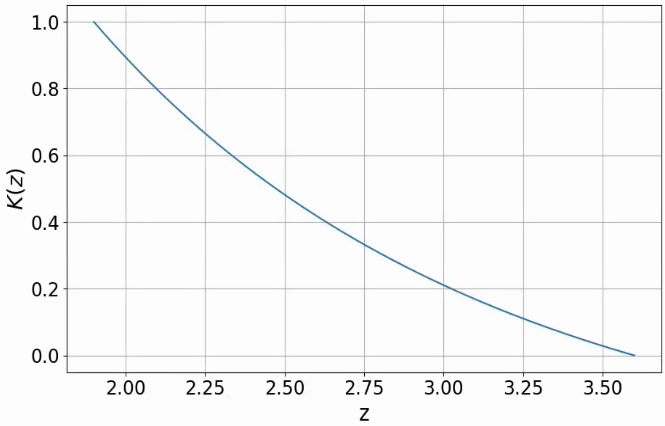
\includegraphics[scale=0.4]{kz}
  \caption{Coefficient $K(z)$ défini dans l'équation~\ref{eq:lognormal_interp}.}
\end{figure}
Les quasars sont ensuites tirés dans chaque voxcell, avec une probabilité $P \propto \hat \delta_{QSO}$. Pour ce faire, nous générons un champ $\phi$ aléatoire uniforme entre 0 et 1, et les voxcells pour lesquelles $\phi < N(z) \hat \delta_{QSO}$ hébergent potentiellement un quasar. Le facteur $N(z)$ est un facteur de normalisation. Les quasars dont le redshift est en dehors de l'intervalle $[\num{1.8}; \num{3.6}]$ sont écartés.
% Les quasars dont l'ascension droite est en dehors de l'inverval $[ - \Delta \alpha ; \Delta \alpha]$ et dont la déclinaison est en dehors de l'inverval $[ - \Delta \delta ; \Delta \delta]$ sont aussi écartés.
Les quasars dont l'ascension droite et la déclinaison sont en dehors des intervalles $[ - \Delta \alpha ; \Delta \alpha]$ et $[ - \Delta \delta ; \Delta \delta]$ sont aussi écartés.
L'ascension droite $\alpha$ et la déclinaison $\delta$ du point $(X,Y,Z)$ sont définies comme
\begin{align}
  \label{eq:radec}
  \alpha &= \arctan(\frac{
  \cos(\alpha_0)X - \sin(\delta_0)\sin(\alpha_0)Y + \cos(\delta_0)\sin(\alpha_0)Z
  }{
  - \sin(\alpha_0)X - \sin(\delta_0)\cos(\alpha_0)Y + \cos(\delta_0)\cos(\alpha_0)Z
           }) \; ,\\
  \delta &= \arcsin(\frac{
           \cos(\delta_0)Y + \sin(\delta_0) Z
           }{
           \sqrt{X^2 + Y^2 + Z^2}
           }) \; .
\end{align}
Enfin, grâce au facteur de normalisation $N(z)$, les quasars sont tirés selon la distribution en $z$ prédite pour DESI. Cette distribution est présentée sur la figure~\ref{fig:dndz_qso}. A la fin, nous obtenons environ \num{100} quasars à $z > \num{2.1}$ par degré carré.
\begin{figure}
  \centering
  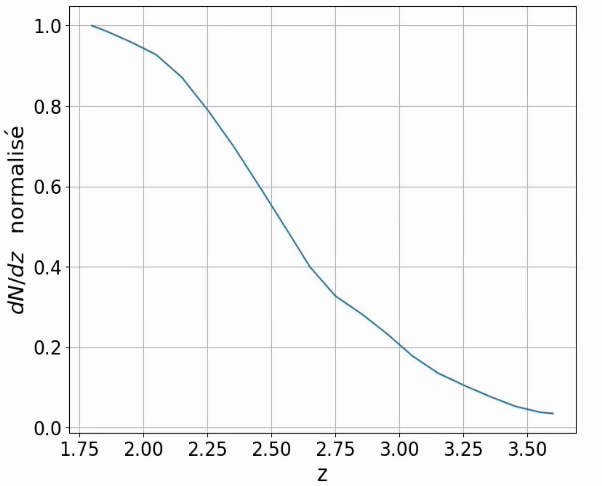
\includegraphics[scale=0.5]{dndz_qso}
  \caption{Distribution normalisée en redshift des quasars tirés dans les mocks.}
\end{figure}

\paragraph{}
Une fois les quasars tirés, nous les déplaçons proportionnellement à leur vitesse $v_{\parallel}$ le long de la ligne de visée. Celle ci est définie comme
\begin{equation}
  v_{\parallel} = \frac{v_x X + v_y Y + v_z Z}{\sqrt{X^2 + Y^2 + Z^2}} \; .
\end{equation}
Ainsi, un quasar situé à une distance $R$ sera replacé le long de la ligne de visé à une distance
\begin{equation}
 R \rightarrow  R + (1+z) \frac{dG}{dz} \frac{1}{H_0 \frac{dG}{dz}(z=0)} v_{\parallel} \; .
\end{equation}
Le facteur $(1+z)$ vient de la conversion des distances en distances comobiles. Une fois tous les quasars déplacés, leur redshift est recalculé, puis ils sont stockés dans un catalogue.


\subsection{Création des lignes de visée}
A cette étape, nous disposons d'un catalogue de quasars, corrélé avec le champ de densité $\delta_{matière}$ qui sera utilisé pour construire l'absorption \lya{}. Nous pouvons donc créer les lignes de visées à partir de chaque quasar, et interpoler le champ de densité le long de celles-ci.
Dans un premier temps, nous commençons par créer le vecteur en longueurs d'onde observées, sur lequel sera interpolé le champ de densité. Nous choisissons une taille de pixel $d_{pix} = \SI{0.2}{\perh\Mpc}$. Les limites $\num{1.8} < z < \num{3.6}$ en redshift se traduisent par des limites $\num{3403.876} < \lambda < \SI{5592.082}{\angstrom}$ sur la longueur d'onde observée. Nous ajoutons la limite basse des spectrographes de DESI : $\lambda_{min} = \SI{3530}{\angstrom}$, que nous réduisons afin d'inclure certains métaux dans les forêts (voir ~\ref{prov}). Les longueurs d'onde observées couvrent donc $\num{3476.1877} < \lambda < \SI{5591.566}{\angstrom}$ à l'aide de \num{6524} pixels.

Une fois ce vecteur en longueur d'onde obtenu, nous le positionnons dans les boîtes afin de construire la ligne de visée à partir de chaque quasar.
% pour chaque quasar, nous calculons la position $(X,Y,Z)$ de chaque pixel.
D'abord, le pixel $\lambda_{QSO} = (1+z_{QSO}) \lambda_{\mathrm{Ly}\alpha}$ est placé à la position $(X_{QSO}, Y_{QSO}, Z_{QSO})$ du quasar, et le vecteur est dirigé vers l'observateur. Puis, pour chaque pixel $i$ entre $\lambda_{min} = \num{3476.1877}$ et $\lambda_{QSO}$, la position $(X_i, Y_i, Z_i)$ du pixel est déterminée.
Le champ est alors interpolé puis lissé. Pour chaque pixel, nous considérons les voxcells appartenant au cube de 7 voxcells de côté, centré sur le voxcell dans lequel se trouve le pixel. Ceci représente donc \num{343} pixel à interpoler puis lisser.
Le pixel $i$ est alors donné par
\begin{equation}
  \delta_i = \sum_{j=0}^{342}  \frac{\delta(\vec r_j) \mathrm{e}^{\frac{-(\vec r_j - \vec r_i)^2 }{ \sigma_j^2}}}{\sigma_j^2} \; ,
\end{equation}
où $\vec r_j$ est la position du voxcell $j$, $\vec r_i$ celle du pixel $i$, $\delta$ est le champ à interpoler, et enfin $\sigma^2 = 2 d_{cell}^2$ est la largeur du lissage gaussien appliqué. Ce lissage est nécessaire afin d'éviter le crénelage aux petites échelles.
Ce calcul est effectué pour tous les pixels qui vérifient $\lambda_i < \lambda_{QSO}$, pour chaque quasar. Les champs interpolés sont le champ $\delta_{matière}$ utilisé pour construire l'absorption \lya{}, les trois champs de vitesse utilisés pour ajouter les RSD aux DLA tirés dans chaque ligne de visée (voir section~\ref{prov}), et les six champs de gradient de vitesse afin d'ajouter les RSD au champ \lya{}.


\subsection{De la densité à l'absorption}
Une fois les lignes de visés interpolées, nous pouvons transformer le champ de densité en absorption \lya{}. Ceci est fait via la formule FGPA :
\begin{equation}
F = \exp( - a(z) \mathrm{e}^{b(z) G(z) \delta}) ;.  
\end{equation}



\bibliography{../source/library}
\end{document}
